\documentclass{article} % \documentclass{} is the first command in any LaTeX code.  It is used to define what kind of document you are creating such as an article or a book, and begins the document preamble

\usepackage{amsmath} % \usepackage is a command that allows you to add functionality to your LaTeX code
\usepackage{graphicx} % allows for images to be added to the latex document
\usepackage{tabularx}
\usepackage[T1]{fontenc}
\usepackage[ddmmyyyy]{datetime}
\usepackage[australian,american]{babel}

\usepackage{hyperref} % allows for hyperlinks to be added to the document
\hypersetup{
    colorlinks,
    citecolor=black,
    filecolor=black,
    linkcolor=black,
    urlcolor=black,
    pdftitle={Research},
    pdfpagemode=FullScreen
}

\usepackage[
backend=biber,
style=numeric-comp,
sorting=ynt
]{biblatex} %Imports biblatex package
\addbibresource{references.bib} %Import the bibliography file

\graphicspath{{../pdf/}{./research_images}}

\title{Research} % Sets article title
\author{Sean Groenenboom \and Seger Sars \and Siem Vermeulen \and Angel Villanueva \and Ronan Vlak} % Sets authors name
\date{\today} % Sets date for date compiled
\newpage
\begin{document}

\maketitle % creates title using information in preamble (title, author, date)
\newpage

\tableofcontents % creates a table of contents
\newpage

\section{Game speed}
Movement is a very important part of any game, but how is movement calculated accurately across different computers?
Different computers have different internals and thus run games with differing performance.
One computer might be able to run the games at 60FPS, but another can only run the game at 30FPS.
How can you make sure that both users have the exact same experience despite the difference in render speed.
A difference in render speed is shown in \autoref{fig:TimeBetweenFramesDisplayed} below.
\begin{figure}[h!]
	\centering
	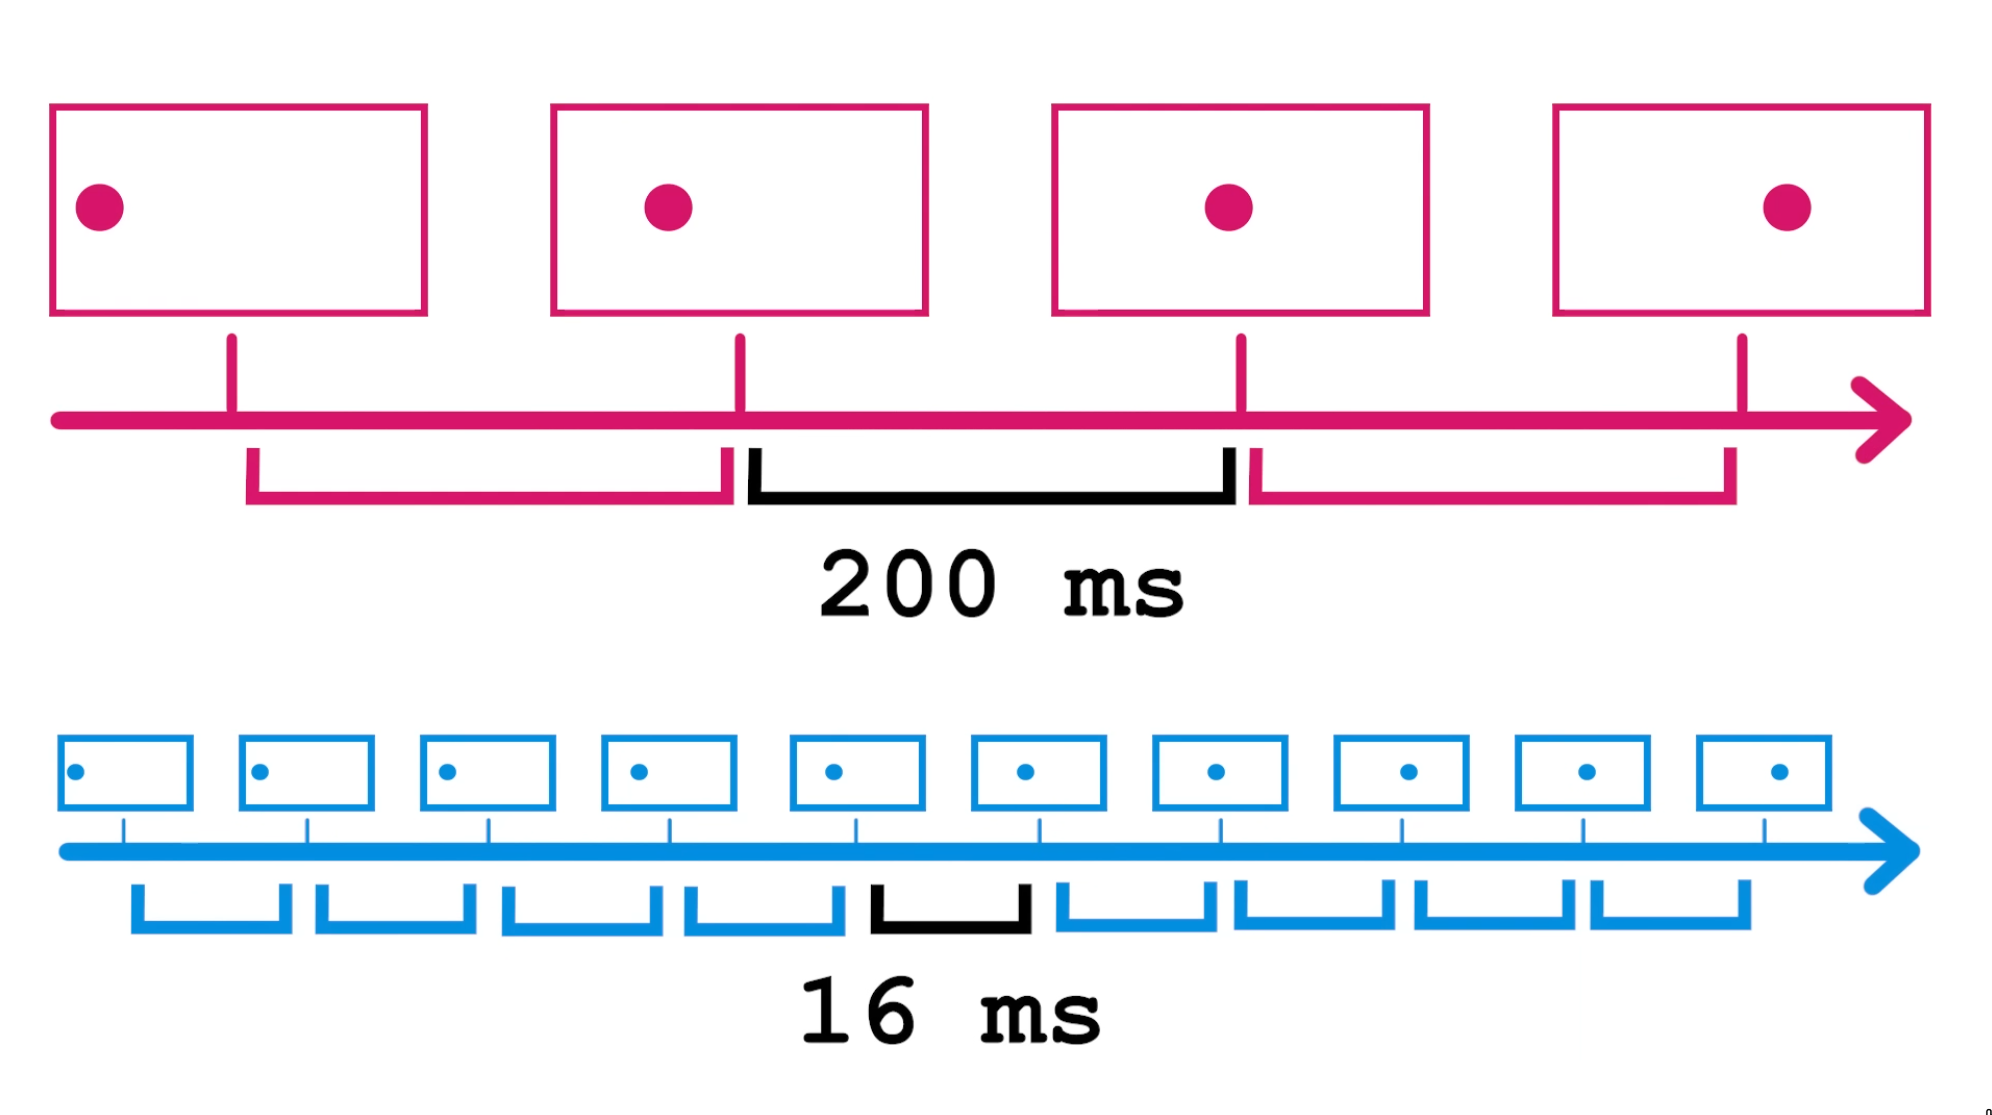
\includegraphics[width=0.8\textwidth]{time_between_frames.png}
	\caption{Time between frames displayed}
	\label{fig:TimeBetweenFramesDisplayed}
\end{figure}

\subsection{Potential problems}
A standard game loop runs one time each frame, before the frame is rendered.
The game loop is responsible for handling all the movement in the game, like moving the player.
If the game runs at 60FPS the game loop will be run 60 times each second.
\newline\newline
The following formula could be used to move the player each game loop iteration:
\newline
playerPosition.x = playerPosition.x + 10
\newline\newline
If this formula would be used to move the player, when running at 60PFS, the player would move 600 units of length each second.
But if the game was running at 30FPS, the player would only move 300 units each second.
So the player with 60FPS is considerably faster than the one with 30FPS.
This is of course, not ideal, as a game developer you want everyone to move at the same speed despite the computer it is run on.
The difference in elapsed distance is also shown in \autoref{fig:DifferenceInElapsedDistance} below.
\begin{figure}[h!]
	\centering
	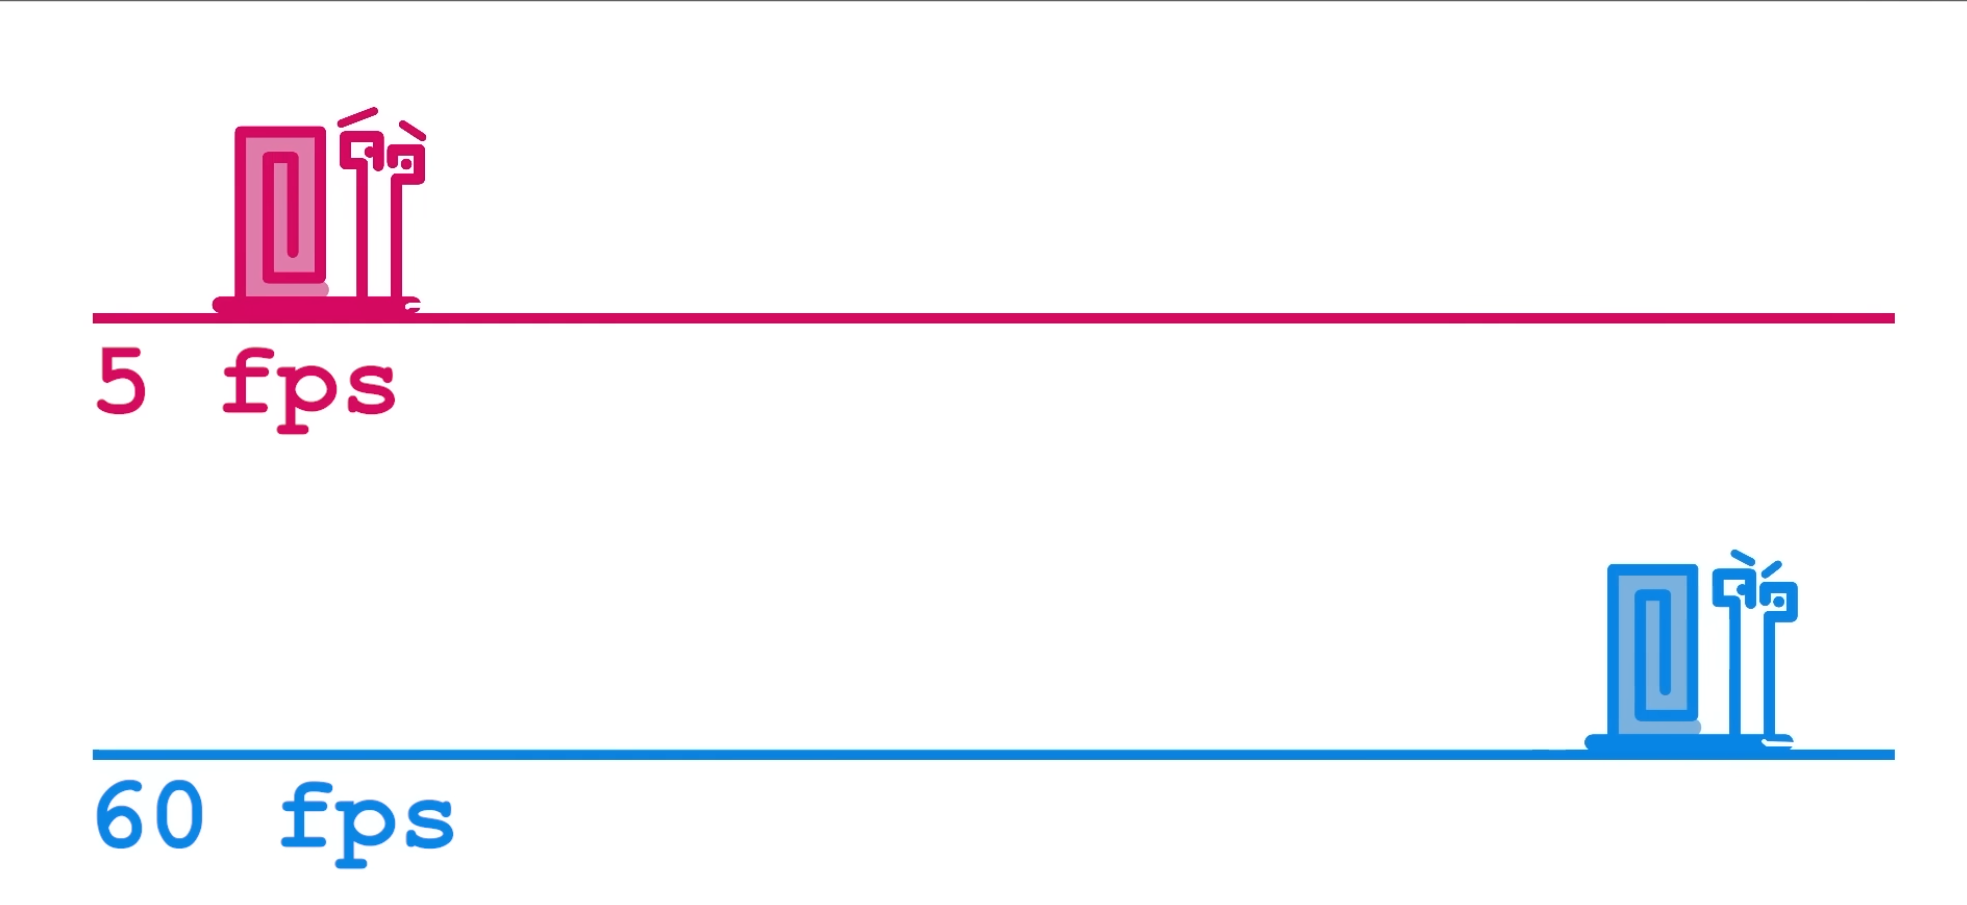
\includegraphics[width=0.8\textwidth]{difference_in_distance.png}
	\caption{Difference in elapsed distance}
	\label{fig:DifferenceInElapsedDistance}
\end{figure}

\subsection{Possible solutions}
There are two common solutions that help alleviate this problem, adjusting the movement speed relative to the FPS or making sure to handle movement in a fixed update loop that is guaranteed to run at a certain amount of cycles each second.

\subsubsection{Fixed update}
A solution to the differing movement speeds between computers, is to create a lightweight time based interrupt, often referred to as FixedUpdate, to handle all movement.
It is important that the FixedUpdate function is very small, otherwise the FixedUpdate could be too slow to be called at a constant rate each frame, defeating the purpose of the FixedUpdate.
In \autoref{fig:FixedUpdateView} below it is shown how times between different rendered frames can vary, while the FixedUpdate is called at a constant rate, where the small black bar represents the duration of the FixedUpdate function.
\begin{figure}[h!]
	\centering
	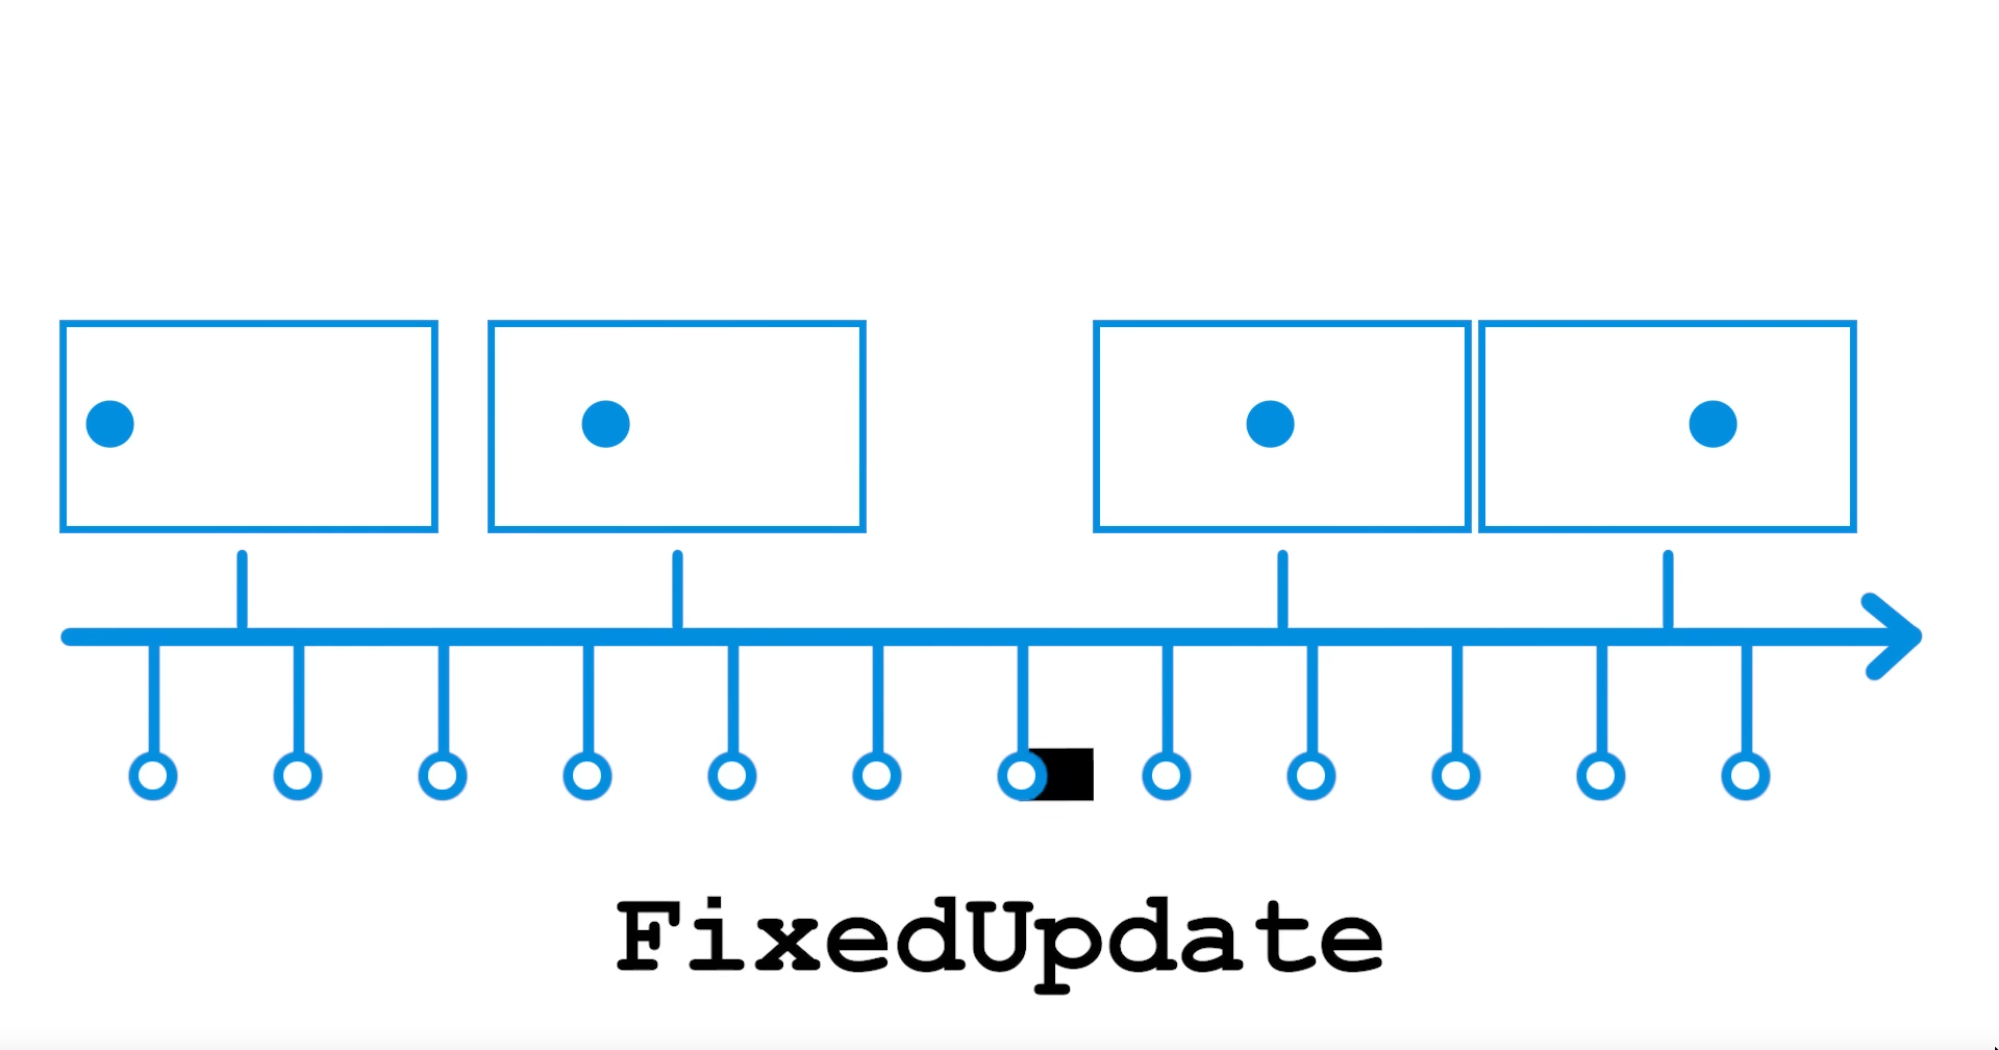
\includegraphics[width=0.6\textwidth]{fixed_update_explanation.png}
	\caption{Fixed update view}
	\label{fig:FixedUpdateView}
\end{figure}
\newline
If you were to use the same formula to calculate the player movement as before, it would now show constant movement between computers.

\subsubsection{Delta time}
Another solution to the differing speeds between computers, is to make the added distance when moving the player relative to the last time distance was added to the player.
Keeping track of every time movement is added to an object is not very efficient so this is solved in a slightly different manner.
So this means the formula would look like this:
\newline
playerPosition.x = playerPosition.x + (10 * deltaTime)
\newline
This uses the deltaTime variable to make the movement relative to the last time the movement was calculated.
\newline\newline
The deltaTime variable is calculated by the game engine and is globally accessible.
The game engine measures the time between the previous frame and the frame before, then assigns that value to the deltaTime variable.
This process is shown in \autoref{fig:DeltaTimeValueWhenUsingVariable}  below where the black square is the place deltaTime is used and the 0.14 is the time it took for the previous frame to render.
\begin{figure}[h!]
	\centering
	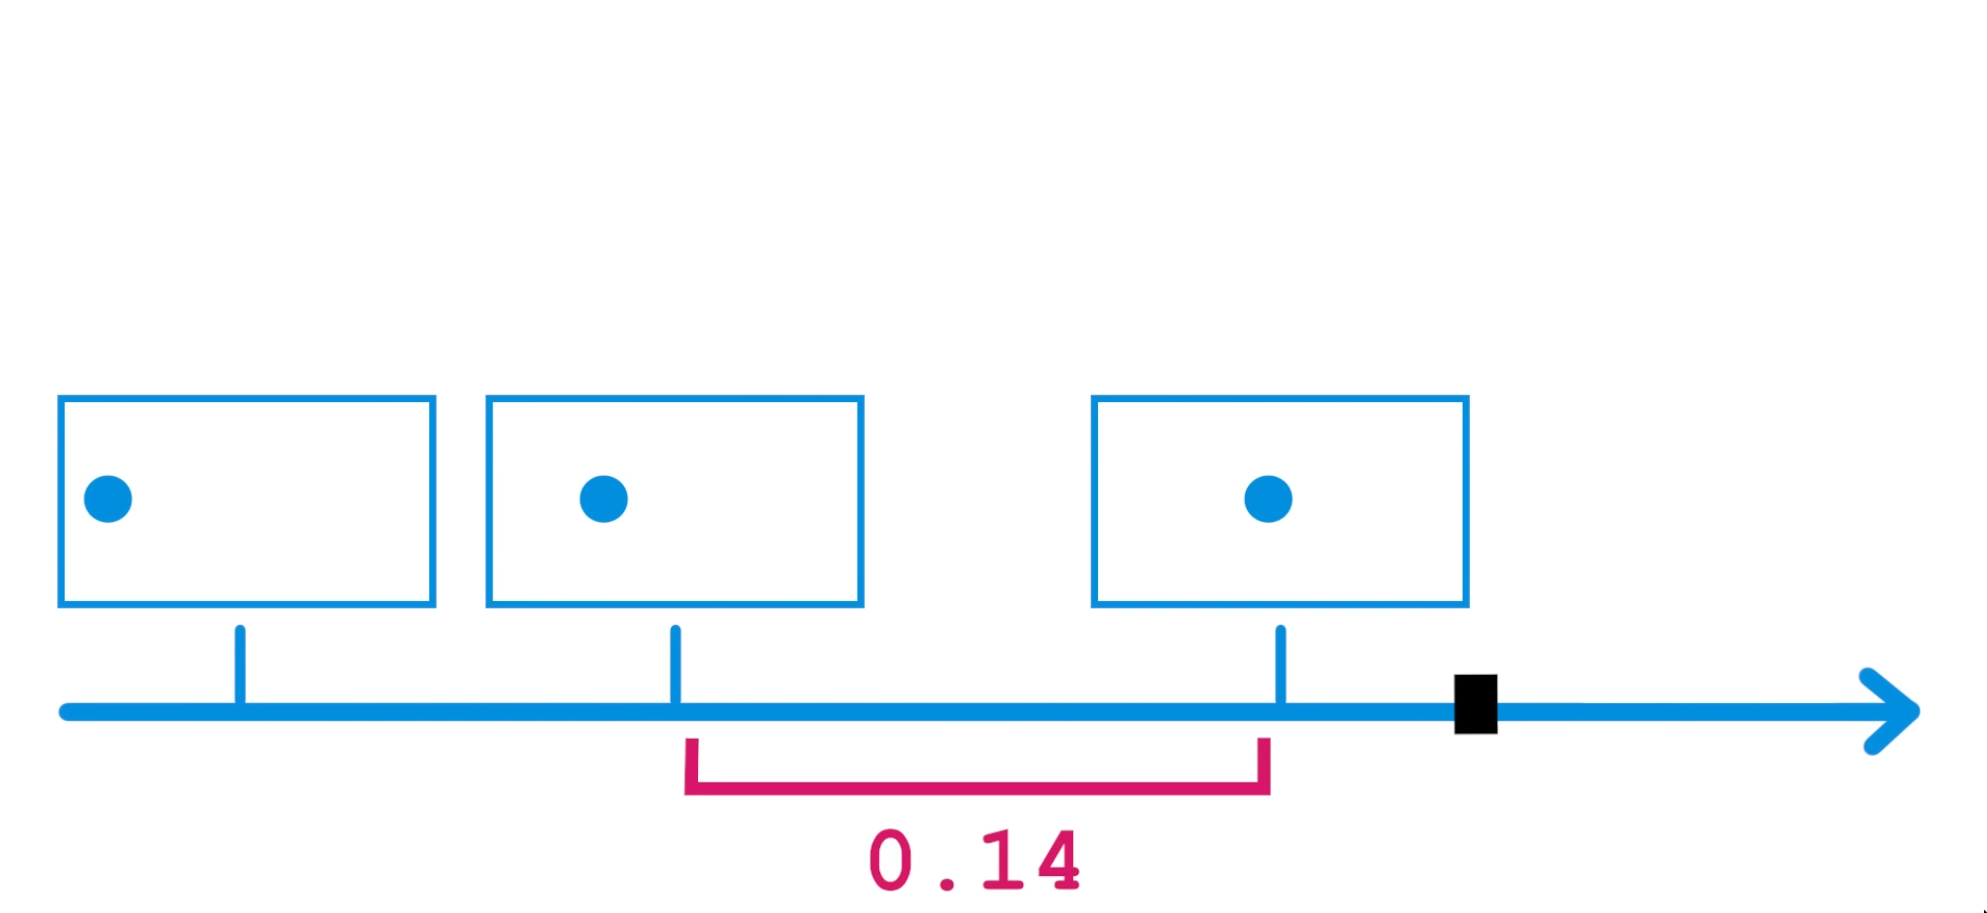
\includegraphics[width=0.6\textwidth]{used_deltatime_when_using_variable.png}
	\caption{deltaTime value when using variable}
	\label{fig:DeltaTimeValueWhenUsingVariable}
\end{figure}
\newline
Because deltaTime is used while rendering a frame, it is not possible to know how long it takes to render the rest of the frame.
This is why the value for the previous frame is used, although this means the deltaTime value lags behind by one frame, the delay is not noticable in most situations.

\newpage


\section{2D rendering}
The game engine has to be able to display and render images on screen.
The game engine will support 2D games, but how does the game engine render images to the screen?

\subsection{SDL2} \label{SDL2}
A simple way to get graphics working in you own custom application is to use a graphics library.
One of the most used simple 2D graphics libraries is SDL2 \cite{sdl2}.
SDL2 is a library written in C that allows the user to have very easy and lightweight cross-platform rendering capabilities.
SDL2 handles most things, so the user can start SDL2 and load and display images, without having to deal with the OS or GPU.
SDL2 does not only handle rendering images but is also capable of managing audio, keyboard, mouse and joystick, allowing for easy user input and audio management across different platforms.

\subsubsection{SDL2 POC}
For the purpose of research a SDL2 POC was created. In this POC the basics of window, renderer and texture creation are covered.
The POC is an application in which an image could be moved across the screen by using the w,a,s and d, keys.
A screenshot of the POC can be seen in \autoref{fig:poc_SDL2}.

\begin{figure}[h!]
	\centering
	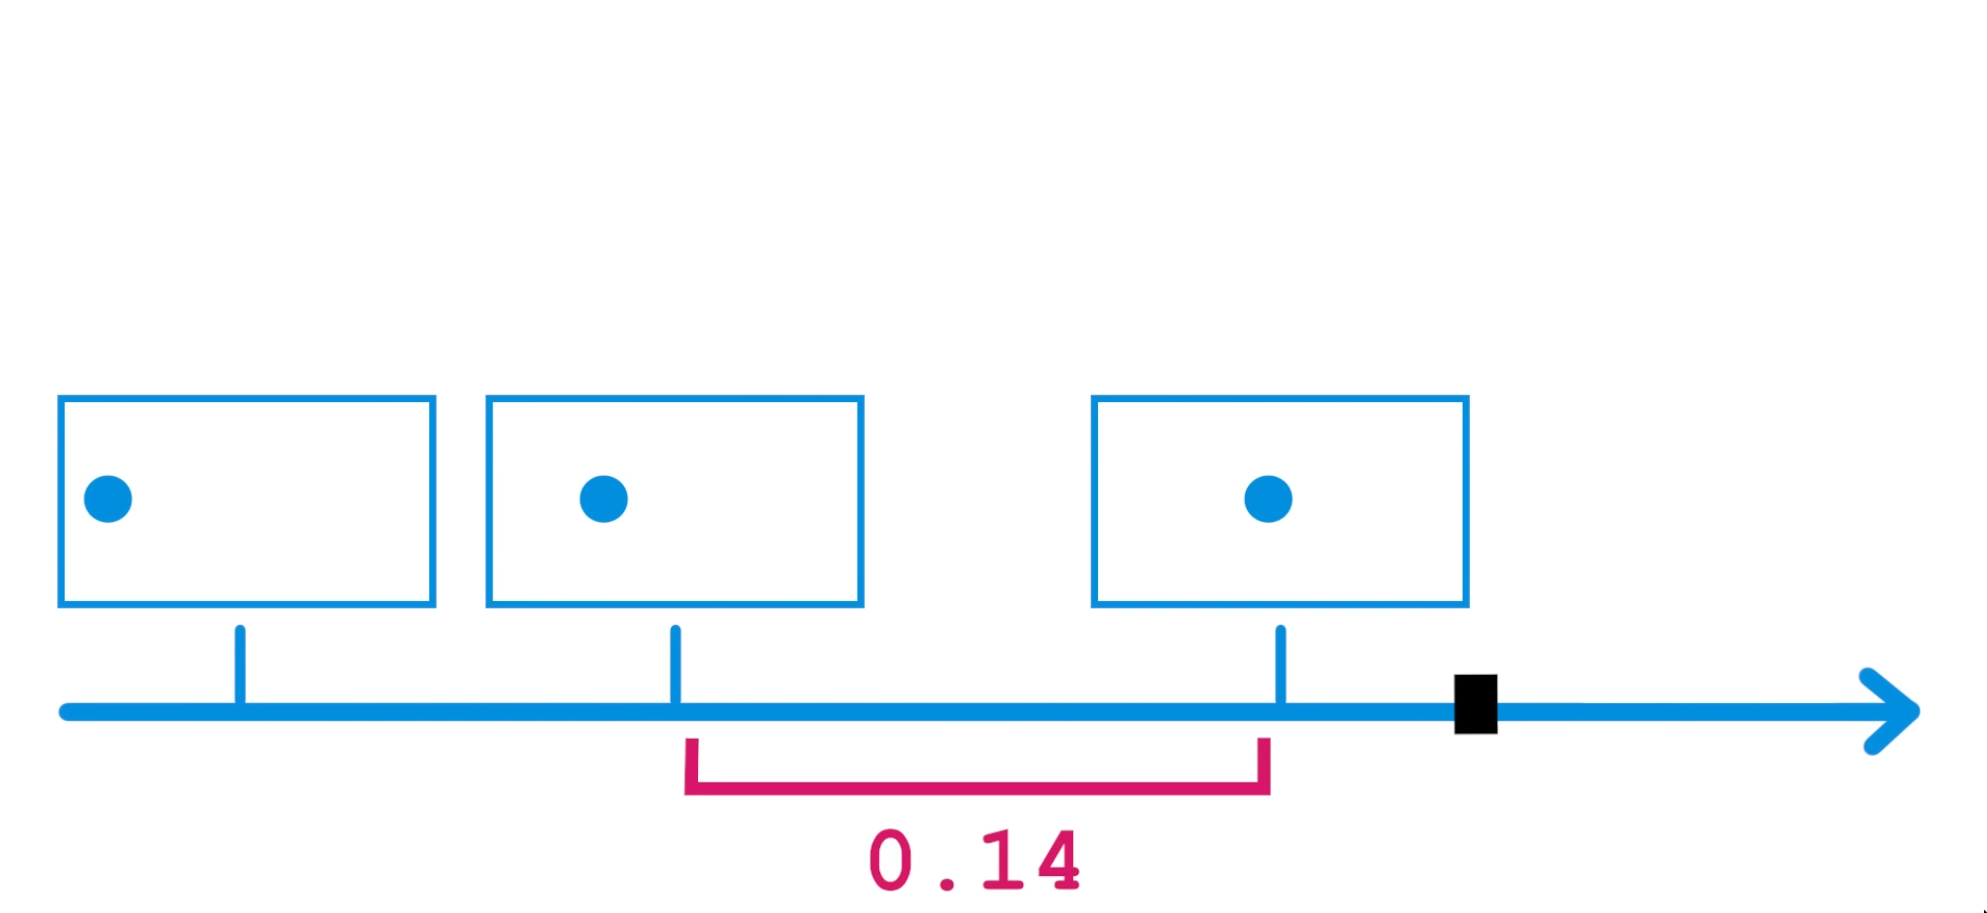
\includegraphics[width=0.7\textwidth]{pos_SDL2_screenshot.png}
	\caption{Screenshot of SDL2 POC}
	\label{fig:poc_SDL2}
\end{figure}

\subsection{Cairo}
Like SDL2 Cairo \cite{cairo}  offers a library written in C that allows the user to render text and images to the screen in a simple way.
Unlike SDL2 Cairo does not offer any access to sound, keyboard, mouse and joystick.
Cairo does not offer these features because the library is meant to be graphics only and as small as possible.

\subsection{OPENGL}
OPENGL \cite{opengl} is not a graphics library but is a shader language, which means that is it a programming language that is compiled to run on the GPU for rendering graphics.
Libraries like SDL2 \cite{sdl2} use OPENGL to render the textures to the screen.
Directly working with OPENGL gives the developer exact control over the render process, textures and effects on screen.
But this exact control comes with way more needed knowledge and development time than using SDL2 which has all the GPU related code under the hood.

\newpage


\section{Sprites and Textures}
Sprites and textures are very important in games, they convey the location and look of most in-game objects.
They are responsible for animations in most 2D games, by showing sprites in a certain order to mimic movement and thereby showing animations and transformations.

\subsection{Storing sprites and animations}
Sprites are usually stored in .png files because they allow for transparent pixels and have lossless compression.
When storing a large amount of sprites of similar size and function, they are usually grouped into sprite sheets, which are large png images that consist of all sprites set beside each other in a grid pattern.
Sprite sheets have animations for certain objects grouped together so they are accessible by consecutive grid coordinates.
Sprite sheets also have the added benefit of less files in a project, because an entire characters sprites can be on a single sprite sheet.
An example of a simple sprite sheet was given below in \autoref{fig:example_sprite_sheet}, in the figure a running animation of the character is depicted.
So in this example a large amount of sprites were created to create a smooth running animation but because they are all on the same sprite sheet the entire animation is stored in a single file.
\begin{figure}[h!]
	\centering
	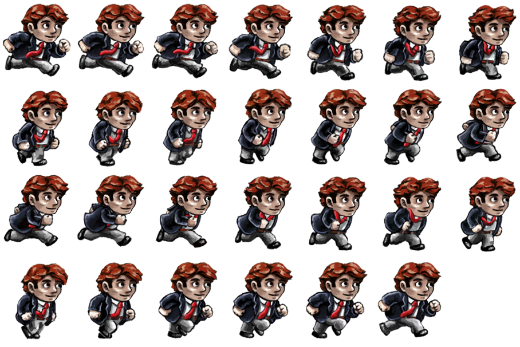
\includegraphics[width=0.2\textwidth]{example_sprite_sheet.png}
	\caption{Example sprite sheet}
	\label{fig:example_sprite_sheet}
\end{figure}

\subsection{Sprite sheet grid structure}
Sprite sheets are organized in a grid pattern.
Because all sprites are the same size the image can be divided into grid coordinates by dividing the image width by the sprite width.
In this way all sprites are able to be selected by choosing x and y coordinates and then extracting that certain part of the image.
A clear grid structure is also shown in \autoref{fig:example_sprite_sheet}.

\subsection{Showing animations}
When trying to show the animation depicted in \autoref{fig:example_sprite_sheet} it is important that the image shown to the player alternates between the images in the sprite sheet.
The speed of alternating between the images is dependent on how fast the animation is supposed to be playing.
Often times when movement between individual frames is low, the time between frames is also low.
Because objects like a player require more animations like standing, walking and jumping, it is important that more than one animation can be linked to an object and that it is possible to switch between those animations.
In extensive game engines switching between animations is handled by an animation system, animations systems are explained further in the Animation systems section.

\subsection{Animation systems}
An animation system in a game engine is the system that manages the transitions between different animations on the same object.
An engine like Unity \cite{unity} has an entire graphical animation system built into the engine like shown in \autoref{fig:unity_animation_system_overview}.
With the graphical animation system that Unity possesses it is possible to define animations, drag and drop them into the animation controller and set transition conditions.
After the initial setup, the animation system switches the shown animation and sprite automatically.

\begin{figure}[h!]
	\centering
	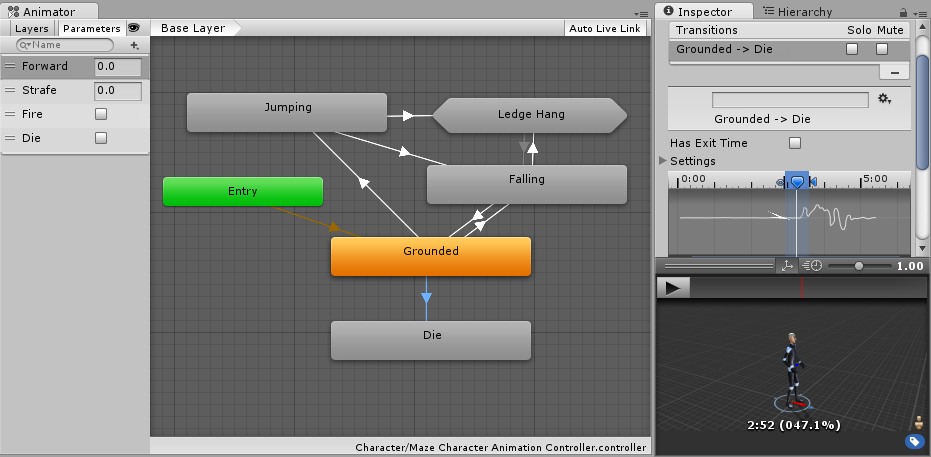
\includegraphics[width=0.9\textwidth]{unity_animation_system_overview.png}
	\caption{Unity animation system overview}
	\label{fig:unity_animation_system_overview}
\end{figure}

\subsection{Sprite atlases}
A sprite atlas class is a software component designed to handle and manage sprite sheets.
This class enables the dissection of a sprite sheet into individual sprites or animations by taking the sheet as input and logically dividing it based on specified parameters like frame width, height, and animation sequences.
By organizing and extracting these individual frames, the sprite atlas class simplifies the process of managing multiple sprites for character animations, user interface elements, or other game assets.

\newpage

\section{Multiplayer}
Multiplayer is an important aspect of gaming. It is not necessary for a game to work, but it can greatly enhance the experience.
\subsection{Models}
There are multiple multiplayer models each with their own advantages and disadvantages. \cite{Kroupp_2024}

\subsubsection{Client-Server Model}
The \textit{client-server} model is one of the most widely used architectures for multiplayer games. In this model, a server hosts the game world, and clients (players) connect to it. The server is considered authoritative, managing the game state and ensuring consistency across all clients.

\textbf{Advantages}
\begin{itemize}
	\item Ensures a consistent and authoritative game state.
	\item Reduces the risk of cheating, as the server controls the game logic.
	\item Scalable for large games (e.g., MMOs).
\end{itemize}

\textbf{Challenges}
\begin{itemize}
	\item Requires a reliable and performant server, which adds complexity and cost.
	\item Introduces latency between clients and the server, which can affect gameplay responsiveness.
\end{itemize}

\subsubsection{Peer-to-Peer (P2P) Model}
In the \textit{peer-to-peer} model, all players (peers) are directly connected to each other, and the game state is shared among them. Each peer has equal authority over the game, which can make synchronization and consistency more difficult to maintain.

\textbf{Advantages}
\begin{itemize}
	\item Simple to implement for small-scale games with a limited number of players.
	\item No need for a dedicated server, reducing costs.
\end{itemize}

\textbf{Challenges}
\begin{itemize}
	\item Difficult to ensure game state consistency across peers.
	\item Susceptible to cheating, as each peer has authority.
	\item Latency and synchronization issues are harder to manage.
\end{itemize}

\subsubsection{Authoritative Server with Client-Side Prediction}
This model combines the \textit{client-server} approach with \textit{client-side prediction}. The server remains authoritative, but clients predict the outcome of their actions while awaiting confirmation from the server. This reduces the apparent latency for the player.

\textbf{Advantages}
\begin{itemize}
	\item Provides a smoother and more responsive experience for players.
	\item Retains the security and consistency of a server-authoritative system.
\end{itemize}

\textbf{Challenges}
\begin{itemize}
	\item Complex to implement, requiring careful handling of discrepancies between predicted and actual outcomes.
	\item Still subject to latency, although mitigated by prediction.
\end{itemize}

\subsubsection{State Synchronization}
In \textit{state synchronization}, the server periodically sends the full game state to clients, ensuring that all players have a consistent view of the game world.

\textbf{Advantages}
\begin{itemize}
	\item Simple to implement for games where maintaining a consistent game state is critical, such as strategy or turn-based games.
	\item Ensures that all clients are synchronized with the server.
\end{itemize}

\textbf{Challenges}
\begin{itemize}
	\item Can be bandwidth-intensive, especially for games with a large or complex game state.
	\item Latency can lead to noticeable delays in the game state being updated on clients.
\end{itemize}

\subsubsection{Event-Driven Networking}
\textit{Event-driven networking} focuses on sending specific events (e.g., player actions) rather than the entire game state. Clients process these events and update their local game state accordingly.

\textbf{Advantages}
\begin{itemize}
	\item More efficient in terms of bandwidth, as only small packets of information are transmitted.
	\item Suitable for games with frequent, small state changes, such as mobile or social games.
\end{itemize}

\textbf{Challenges}
\begin{itemize}
	\item Requires careful ordering and processing of events to ensure consistency.
	\item Can be difficult to implement for games with complex interactions.
\end{itemize}

\subsubsection{Hybrid Models}
Many games use a \textit{hybrid} approach, combining aspects of different multiplayer models to optimize performance, scalability, and security. For example, a game might use the client-server model for general game logic but implement peer-to-peer connections for specific tasks like voice chat or trading.

\textbf{Advantages}
\begin{itemize}
	\item Offers flexibility to tailor the multiplayer system to different aspects of the game.
	\item Allows for optimization of performance and scalability where needed.
\end{itemize}

\textbf{Challenges}
\begin{itemize}
	\item Increases complexity, requiring careful design to ensure all components work seamlessly together.
	\item May require more effort to maintain and debug.
\end{itemize}

\subsection{Tools}
The development of multiplayer games requires specialized tools and frameworks to ensure smooth,
real-time communication between players, game servers, and clients. Whether it's managing the networking stack, handling player synchronization, or reducing latency,
choosing the right multiplayer tool is crucial to the success of any game. This chapter explores the most commonly used multiplayer tools for professional game developers,
followed by a section specifically aimed at student developers using C++.

\subsubsection{Commonly Used Multiplayer Tools for Professional Developers}
Professional game developers often need multiplayer tools that are scalable, feature-rich, and easy to integrate with large, complex projects. The tools listed below are widely used in the industry for various types of multiplayer games.

\paragraph{Unity} (with Netcode for GameObjects or Mirror)
is one of the most popular game engines for both 2D and 3D game development,
and it provides several options for multiplayer networking.
\\
\textbf{Advantages}:
\begin{itemize}
	\item Extensive documentation and community support.
	\item Tight integration with Unity's development workflow.
	\item Multiple networking solutions, including Netcode for GameObjects (official) and Mirror (open-source).
\end{itemize}
\textbf{Disadvantages}:
\begin{itemize}
	\item Limited scalability for very large multiplayer projects.
	\item Mirror, while simple, may require additional setup for complex use cases.
\end{itemize}

\paragraph{Unreal Engine} (with Unreal Networking) Unreal Engine,
a high-end game engine used in AAA titles, includes built-in support for multiplayer via its advanced networking framework.
\\
\textbf{Advantages}:
\begin{itemize}
	\item Built-in support for replication and remote procedure calls (RPCs).
	\item Highly scalable, suitable for large multiplayer games.
	\item Excellent graphics and physics, suitable for visually intensive games.
\end{itemize}
\textbf{Disadvantages}:
\begin{itemize}
	\item Steep learning curve, especially for new developers.
	\item Resource-intensive, requiring powerful hardware for development.
\end{itemize}

\paragraph{Photon Engine} is a cloud-based multiplayer framework designed to scale from small indie games to large multiplayer experiences.
\\
\textbf{Advantages}:
\begin{itemize}
	\item Cloud-hosted and scalable.
	\item Supports both authoritative server and peer-to-peer networking models.
	\item Easy integration with Unity and Unreal Engine.
\end{itemize}
\textbf{Disadvantages}:
\begin{itemize}
	\item Requires a Photon cloud subscription for larger projects.
	\item May add latency depending on the geographical location of servers.
\end{itemize}

\paragraph{Godot} (with ENet or Nakama) Godot is a free,
open-source game engine that supports both 2D and 3D games.
It has a lightweight networking stack using libraries such as ENet or Nakama.
\\
\textbf{Advantages}:
\begin{itemize}
	\item Free and open-source, ideal for indie developers.
	\item Lightweight and fast, especially for 2D games.
	\item Community-driven development and support.
\end{itemize}
\textbf{Disadvantages}:
\begin{itemize}
	\item Lacks the advanced tools found in Unity or Unreal for larger games.
	\item Smaller community compared to other engines.
\end{itemize}

\paragraph{PlayFab} is a backend service for multiplayer games that provides tools like player authentication, leaderboards, and matchmaking.
\\
\textbf{Advantages}:
\begin{itemize}
	\item Fully managed backend service, reducing server-side complexity.
	\item Integrates with multiple game engines.
	\item Scales for small and large games.
\end{itemize}
\textbf{Disadvantages}:
\begin{itemize}
	\item Requires an active subscription for large-scale use.
	\item May not offer the same level of control as self-hosted solutions.
\end{itemize}

\subsubsection{Multiplayer Tools for C++ Student Developers}
For student developers working with C++,
multiplayer tools must be lightweight, flexible, and simple to integrate.
Below are some commonly used tools for networking in C++ game projects.

\paragraph{ENet} is a reliable UDP-based networking library designed for real-time multiplayer games.
\\
\textbf{Advantages}:
\begin{itemize}
	\item Lightweight and easy to integrate.
	\item Provides reliable UDP, packet sequencing, and fragmentation.
	\item Perfect for real-time, fast-paced multiplayer games.
\end{itemize}
\textbf{Disadvantages}:
\begin{itemize}
	\item Does not offer high-level features such as matchmaking or player authentication.
	\item Requires manual implementation of game-specific features like lag compensation.
\end{itemize}

\paragraph{RakNet} (or SLikeNet) is a feature-rich networking engine designed for multiplayer games. SLikeNet is its actively maintained fork.
\\
\textbf{Advantages}:
\begin{itemize}
	\item Supports advanced features such as NAT punch-through, RPCs, and object replication.
	\item Cross-platform, with easy integration into various game engines.
	\item Highly suitable for both small and large multiplayer games.
\end{itemize}
\textbf{Disadvantages}:
\begin{itemize}
	\item More complex to learn and use compared to simpler libraries like ENet.
	\item RakNet’s development has slowed, although SLikeNet remains maintained.
\end{itemize}

\paragraph{asio} (Boost.Asio or standalone) is a general-purpose C++ networking library that supports both TCP and UDP communication and focuses on asynchronous I/O.
\\
\textbf{Advantages}:
\begin{itemize}
	\item Powerful and flexible, allowing developers to build custom networking solutions.
	\item Works well for both small-scale and large-scale projects.
	\item Supports asynchronous programming, which is crucial for multiplayer games.
\end{itemize}
\textbf{Disadvantages}:
\begin{itemize}
	\item Low-level, so developers need to implement most game-specific networking logic.
	\item Steeper learning curve due to its focus on concurrency and asynchronous programming.
\end{itemize}

\paragraph{KCP} (A Fast and Reliable UDP Protocol) KCP is a reliable and efficient UDP-based protocol for low-latency multiplayer games.
\\
\textbf{Advantages}:
\begin{itemize}
	\item High-performance, optimized for low-latency environments.
	\item Easy to integrate with existing networking systems.
\end{itemize}
\textbf{Disadvantages}:
\begin{itemize}
	\item Lacks higher-level features such as matchmaking, lobbies, or session management.
	\item Requires developers to implement their own game logic on top of the protocol.
\end{itemize}

\paragraph{Steamworks SDK} is a set of tools and services provided by Valve for games that are distributed via the Steam platform. It provides networking solutions as well as other features such as achievements, leaderboards, and user authentication.
\\
\textbf{Advantages}:
\begin{itemize}
	\item \textbf{Integration with Steam}: Provides seamless integration with the Steam platform, including achievements, leaderboards, and Steam Cloud.
	\item \textbf{Peer-to-peer and server-based networking}: Supports both peer-to-peer connections and server-authoritative networking models.
	\item \textbf{Matchmaking and lobbies}: Built-in support for lobbies, matchmaking, and friend invites, making it easier to manage multiplayer game sessions.
\end{itemize}

\textbf{Disadvantages}:
\begin{itemize}
	\item \textbf{Limited to Steam}: Only useful for games distributed via Steam, limiting its use for cross-platform or non-Steam games.
	\item \textbf{Requires Steam API knowledge}: Developers need to be familiar with Steam's API, which adds complexity to the development process.
\end{itemize}

\newpage

\section{AI}
\subsection{Commonly Used AI Techniques in Games}

Artificial Intelligence (AI) plays an essential role in game design, affecting the behavior of enemies, NPCs, and other dynamic entities in a game world. Different genres of games utilize AI techniques that cater to specific needs, such as pathfinding, decision-making, and adapting to player behaviors. This chapter explores some of the most commonly used AI techniques in modern games, ranging from simple, rule-based systems to more advanced, machine-learning-based approaches.

\subsubsection{Finite State Machines (FSM)}

Finite State Machines (FSMs) are one of the most basic but widely used AI techniques in game development. They define a set of states and transitions between them based on events or inputs. For example, an enemy NPC might have states like \textit{idling}, \textit{attacking}, and \textit{fleeing}. When a specific condition is met, such as the player coming within range, the FSM triggers a transition from one state to another.

\textbf{Advantages}:
\begin{itemize}
	\item Simple to implement and understand.
	\item Efficient for handling basic enemy behaviors.
	\item Lightweight with low computational cost.
\end{itemize}

\textbf{Challenges}:
\begin{itemize}
	\item Limited flexibility; complex behaviors require extensive state management.
	\item Difficult to scale as complexity grows, leading to the "state explosion problem." \end{itemize}

\subsubsection{Behavior Trees}

Behavior Trees extend FSMs by introducing a hierarchical decision-making process. They allow for more structured and flexible AI behavior, where agents can prioritize tasks based on conditions, making them well-suited for more sophisticated AI.

\textbf{Advantages}:
\begin{itemize}
	\item More scalable than FSMs, allowing for complex decision-making.
	\item Modular and reusable: parts of the tree can be reused across different entities.
	\item Easier to debug and expand compared to FSMs.
\end{itemize}

\textbf{Challenges}:
\begin{itemize}
	\item More complex to implement and requires more computational resources.
	\item Managing large trees can still become cumbersome in certain cases.
\end{itemize}

\subsubsection{Pathfinding Algorithms}

Pathfinding is a crucial AI component, especially for games with complex environments. The \textit{A*} algorithm is the most popular for real-time games, efficiently finding the shortest path between two points by evaluating the cost of traversing different nodes.

\textbf{Advantages}:
\begin{itemize}
	\item The \textit{A*} algorithm is very efficient and widely supported.
	\item Provides fast and optimal pathfinding solutions for large maps.
\end{itemize}

\textbf{Challenges}:
\begin{itemize}
	\item Can become expensive with large numbers of agents or highly complex maps.
	\item Not suitable for dynamic environments unless paired with other techniques like navigation meshes.
\end{itemize}

\subsubsection{Dynamic Difficulty Adjustment (DDA)}

Dynamic Difficulty Adjustment (DDA) modifies the difficulty of the game in real-time based on player performance. This technique ensures players remain engaged without feeling frustrated or bored, as it adjusts factors like enemy strength or spawn rate.

\textbf{Advantages}:
\begin{itemize}
	\item Keeps gameplay engaging by adapting to player skill levels.
	\item Extends the game's appeal to a broader audience.
\end{itemize}

\textbf{Challenges}:
\begin{itemize}
	\item Requires careful tuning to avoid feeling unfair or too easy.
	\item More complex to implement as it needs real-time analysis of player behavior.
\end{itemize}

\subsubsection{Fuzzy Logic Systems}

Fuzzy Logic Systems introduce a degree of uncertainty and imprecision into AI decision-making, allowing NPCs to make more human-like decisions. Rather than working with strict true/false conditions (like FSMs), fuzzy logic allows for various degrees of truth, which can be useful for situations like deciding an NPC's reaction to danger based on proximity or player actions.

\textbf{Advantages}:
\begin{itemize}
	\item Allows for more natural, human-like decision-making.
	\item Can create more nuanced and dynamic AI behaviors.
\end{itemize}

\textbf{Challenges}:
\begin{itemize}
	\item More difficult to implement and requires fine-tuning to achieve desired results.
	\item Can be computationally expensive depending on the number of variables.
\end{itemize}

\subsubsection{Utility Systems}

Utility Systems rank potential actions based on a numerical evaluation of their desirability. AI agents constantly evaluate various options and choose the one with the highest utility score. This allows for flexible decision-making, where actions like attacking, fleeing, or patrolling can be dynamically prioritized based on the game state.

\textbf{Advantages}:
\begin{itemize}
	\item Highly flexible and capable of handling complex decision-making scenarios.
	\item Easier to scale than FSMs or Behavior Trees.
	\item Allows AI to make more context-sensitive decisions based on multiple factors.
\end{itemize}

\textbf{Challenges}:
\begin{itemize}
	\item Requires careful balancing of utility values to prevent undesired behaviors.
	\item More computationally expensive due to constant evaluation of utility scores.
\end{itemize}

\subsubsection{Machine Learning (ML) Techniques}

Machine Learning (ML) is an emerging field in game AI, where AI agents can learn and adapt based on player behavior or environmental conditions. Techniques such as Neural Networks, Reinforcement Learning, and Genetic Algorithms are being experimented with to create self-learning NPCs that evolve over time.

\textbf{Advantages}:
\begin{itemize}
	\item Capable of producing highly adaptive and unpredictable AI behavior.
	\item Can create AI that personalizes its strategy based on the player's habits.
	\item Reduces the need for manually scripting behaviors.
\end{itemize}

\textbf{Challenges}:
\begin{itemize}
	\item Requires large amounts of data and training, making it computationally expensive.
	\item Difficult to implement and balance, especially in real-time environments.
	\item Behavior may become too unpredictable or less fun for players.
\end{itemize}

\subsubsection{Navigation Meshes (NavMesh)}

Navigation Meshes, or NavMeshes, are used in pathfinding to simplify complex environments by mapping walkable areas. Instead of searching an entire map for a path, an agent can move within predefined regions, making pathfinding more efficient, especially in large or dynamic environments.

\textbf{Advantages}:
\begin{itemize}
	\item Reduces the complexity of pathfinding by limiting the search space.
	\item Efficient for handling dynamic environments and obstacles.
\end{itemize}

\textbf{Challenges}:
\begin{itemize}
	\item Requires upfront preprocessing of the map to generate the NavMesh.
	\item Needs to be updated if the game environment changes frequently.
\end{itemize}

\subsubsection{Steering Behaviors}

Steering Behaviors are used to simulate more organic movements of AI agents in environments, such as flocking, avoiding obstacles, or following the player. These behaviors are especially useful in simulating crowds or large groups of NPCs.

\textbf{Advantages}:
\begin{itemize}
	\item Creates smooth, natural movement patterns.
	\item Useful for dynamic, real-time movement like crowd simulations or NPC interactions.
\end{itemize}

\textbf{Challenges}:
\begin{itemize}
	\item Complex combinations of behaviors can be difficult to manage.
	\item Can require significant fine-tuning to avoid unnatural or jittery movements.
\end{itemize}

\subsection{Commonly Used AI Techniques in 2D Bullet Hell Shooters}

In 2D bullet hell shooters, Artificial Intelligence (AI) takes on a specialized role where the focus is on generating challenging bullet patterns and managing enemy waves. This chapter explores the key AI techniques used in these types of games, including bullet management, enemy behavior, and adaptive strategies that create the signature intensity of bullet hell games.

\subsubsection{Bullet Patterns and Trajectory-based AI}

In bullet hell shooters, the complexity of bullet patterns forms the foundation of the game's difficulty. Bullets follow predefined or procedurally generated trajectories, creating patterns like waves, spirals, or grids. These patterns are often carefully crafted to ensure the player has just enough room to dodge while being overwhelmed by projectiles.

\textbf{Advantages}:
\begin{itemize}
	\item Adds depth and challenge to gameplay through complex bullet patterns.
	\item Bullet patterns can be handcrafted or procedurally generated for variety.
\end{itemize}

\textbf{Challenges}:
\begin{itemize}
	\item Managing numerous bullets can lead to performance issues.
	\item Requires meticulous balancing to prevent the game from becoming too difficult or too easy.
\end{itemize}

\subsubsection{Predictive Targeting}

Some enemies in bullet hell shooters use predictive targeting, where bullets are aimed based on the player's projected movement. This creates a more challenging environment, as players cannot rely solely on dodging but must also outsmart the enemy AI.

\textbf{Advantages}:
\begin{itemize}
	\item Makes the game more challenging and less predictable for players.
	\item Adds a strategic layer to movement and bullet dodging.
\end{itemize}

\textbf{Challenges}:
\begin{itemize}
	\item Can become frustrating for players if overused.
	\item Requires careful balancing to avoid overwhelming the player.
\end{itemize}

\subsubsection{Finite State Machines (FSM) for Boss AI}

Boss AI in bullet hell shooters typically involves multiple phases, each with unique attack patterns and behaviors. Finite State Machines (FSMs) are often used to manage these transitions, allowing for a structured approach to changing behavior based on health thresholds, time-based triggers, or other conditions.

\textbf{Advantages}:
\begin{itemize}
	\item Effective at managing complex boss behaviors and phase transitions.
	\item Easier to implement compared to more advanced AI techniques.
\end{itemize}

\textbf{Challenges}:
\begin{itemize}
	\item Boss AI can become predictable if the FSM is too simple.
	\item Requires additional design effort to balance boss difficulty.
\end{itemize}

\subsubsection{Randomized Bullet Patterns}

Randomization adds variability to the bullet hell experience by altering bullet speed, direction, or spawn points in real time. This can make bullet patterns less predictable, forcing players to stay on their toes and adapt to unexpected changes.

\textbf{Advantages}:
\begin{itemize}
	\item Keeps gameplay fresh and prevents players from memorizing patterns.
	\item Can create unique and unpredictable challenges on each playthrough.
\end{itemize}

\textbf{Challenges}:
\begin{itemize}
	\item Too much randomness can lead to frustrating, unavoidable deaths.
	\item Difficult to balance between unpredictability and fairness.
\end{itemize}

\subsubsection{Adaptive Difficulty AI}

Adaptive difficulty AI adjusts the intensity of enemy waves and bullet patterns based on the player’s performance. For example, if a player is performing well, the AI might increase the number or speed of bullets, while underperforming players might face fewer projectiles.

\textbf{Advantages}:
\begin{itemize}
	\item Helps maintain player engagement by preventing frustration or boredom.
	\item Can create a more personalized and balanced experience for different skill levels.
\end{itemize}

\textbf{Challenges}:
\begin{itemize}
	\item Requires careful tuning to avoid making the game too easy or hard.
	\item May result in less consistent difficulty progression for players who prefer a steady challenge.
\end{itemize}

\subsubsection{Steering Behaviors for Enemy Movements}

Steering behaviors can be applied to enemy movements, allowing them to dynamically dodge player attacks, adjust formations, or group together. This technique can be used to create more intelligent and unpredictable enemies that respond to the player's position in real time.

\textbf{Advantages}:
\begin{itemize}
	\item Creates more fluid and realistic enemy movements.
	\item Enhances the challenge by preventing players from easily predicting enemy movement patterns.
\end{itemize}

\textbf{Challenges}:
\begin{itemize}
	\item Can be difficult to balance, as overly dynamic movements might frustrate players.
	\item Requires additional computational resources to manage real-time movement adjustments.
\end{itemize}

\subsubsection{Pattern Sequencing and Combination}

AI can create bullet patterns by sequencing or combining simpler patterns to generate more complex attacks. By layering waves, spirals, or radial bursts in different sequences, the game can generate intricate attack patterns without needing to design every bullet’s trajectory manually.

\textbf{Advantages}:
\begin{itemize}
	\item Allows for the creation of complex patterns from simpler elements.
	\item Patterns can be customized dynamically to suit different levels or bosses.
\end{itemize}

\textbf{Challenges}:
\begin{itemize}
	\item Combining multiple patterns can make the game harder to debug or balance.
	\item The computational cost of tracking multiple, layered patterns may affect performance.
\end{itemize}

\subsubsection{Wave-based AI for Enemy Generation}

In many bullet hell shooters, enemies are spawned in waves with specific patterns or behaviors. AI can control the timing, frequency, and positioning of these waves to increase the difficulty as the game progresses. Certain waves may have unique bullet patterns or movement behaviors, adding variety to the game.

\textbf{Advantages}:
\begin{itemize}
	\item Helps maintain a steady challenge throughout gameplay.
	\item Provides opportunities for mixing up enemy types and patterns, creating a dynamic experience.
\end{itemize}

\textbf{Challenges}:
\begin{itemize}
	\item Predictable wave structures may reduce long-term replayability.
	\item Wave design requires careful balancing to avoid overwhelming or under-challenging players.
\end{itemize}

\subsubsection{Hitbox-based Collision Detection}

In bullet hell shooters, precise hitbox-based collision detection is critical. AI controls the placement and speed of bullets in ways that take advantage of the player’s hitbox size. The AI must ensure that bullet clusters can be narrowly avoided but still provide a significant challenge.

\textbf{Advantages}:
\begin{itemize}
	\item Creates tight, high-stakes gameplay as players dodge bullets that are near their hitbox.
	\item Encourages skillful play, as players can learn to maneuver through challenging bullet patterns.
\end{itemize}

\textbf{Challenges}:
\begin{itemize}
	\item Can frustrate players if hitboxes are unclear or inconsistent.
	\item Requires precise balancing of bullet speed and placement to avoid unfair deaths.
\end{itemize}

\subsubsection{Procedural Bullet Generation}

Procedural generation techniques are often used to create new and unpredictable bullet patterns in real-time, increasing replayability and variety. This method allows the game to generate complex patterns based on seed values or player inputs.

\textbf{Advantages}:
\begin{itemize}
	\item Increases replayability through unpredictability and variability in bullet patterns.
	\item Reduces the need for hand-crafting every bullet pattern, saving development time.
\end{itemize}

\textbf{Challenges}:
\begin{itemize}
	\item Procedurally generated patterns may lack the precision and design of handcrafted ones.
	\item Balancing can be difficult when bullet patterns are not carefully curated.
\end{itemize}

\subsection{Commonly Used Game Engine Libraries for AI}

Several game engine libraries and tools are available for implementing AI in C++. This chapter explores commonly used libraries that simplify AI development for various game genres.

\subsubsection{OpenSteer}

\textit{OpenSteer} is a library designed for steering behaviors, which are useful in AI for controlling agent movement. It supports behaviors like seeking, fleeing, and evading, making it ideal for games with dynamic agent movement such as real-time strategy games or simulations.

\textbf{Advantages}:
\begin{itemize}
	\item Lightweight and easy to integrate into existing engines.
	\item Provides robust solutions for AI movement and steering behaviors.
\end{itemize}

\textbf{Challenges}:
\begin{itemize}
	\item Primarily focused on steering, limiting its scope for other AI needs.
	\item Not suited for games with more advanced decision-making or pathfinding requirements.
\end{itemize}

\subsubsection{Recast and Detour}

\textit{Recast and Detour} is a combination of libraries that handle navigation mesh generation and pathfinding. Recast builds navigation meshes based on 3D geometry, while Detour is responsible for efficient pathfinding across those meshes.

\textbf{Advantages}:
\begin{itemize}
	\item Provides efficient and scalable navigation solutions for complex environments.
	\item Widely used and supported in both 2D and 3D games.
\end{itemize}

\textbf{Challenges}:
\begin{itemize}
	\item Primarily designed for 3D games, requiring adaptation for 2D environments.
	\item Complex setup compared to simpler AI movement libraries.
\end{itemize}

\subsubsection{Behavior3Cpp}

\textit{Behavior3Cpp} is a C++ library for implementing Behavior Trees. It allows developers to structure complex AI decision-making processes and easily manage hierarchical behaviors.

\textbf{Advantages}:
\begin{itemize}
	\item Powerful for creating complex, reusable AI logic.
	\item More flexible than FSMs, allowing for scalable decision trees.
\end{itemize}

\textbf{Challenges}:
\begin{itemize}
	\item More difficult to learn and implement than basic FSMs.
	\item Requires careful management of large behavior trees to avoid performance issues.
\end{itemize}

\subsection{AI Behavior Libraries for 2D Bullet Hell Shooters in C++ for Students}

Developing a 2D bullet hell shooter in C++ requires robust AI behavior libraries to manage complex tasks like enemy movements, bullet patterns, and decision-making processes. This chapter highlights AI libraries that are specifically designed for behavior modeling in C++ game engines. These libraries provide tools for managing AI decision trees, state machines, and behavior trees, which are essential for controlling enemy actions and bullet trajectories in bullet hell shooters.

\subsubsection{libBehaviour}

\textit{libBehaviour} is a lightweight C++ library focused on implementing behavior trees. Behavior trees are highly structured decision-making models commonly used in games for controlling AI behavior. In bullet hell shooters, \textit{libBehaviour} can be used to control enemy actions, such as attacking, dodging, or changing bullet patterns depending on the player’s movements.

\textbf{Advantages}:
\begin{itemize}
	\item Simple to integrate into custom game engines, with a clean and minimalistic API.
	\item Ideal for students looking to learn about behavior trees and AI decision-making.
	\item Extensible and flexible for use in various AI systems.
\end{itemize}

\textbf{Challenges}:
\begin{itemize}
	\item Lacks more advanced features like dynamic pathfinding or navigation.
	\item Requires additional work to implement complex behaviors in a bullet hell context.
\end{itemize}

\subsubsection{BehaviorTree.CPP}

\textit{BehaviorTree.CPP} is a highly efficient C++ library that allows you to create and manage behavior trees. This library is especially useful for controlling complex AI behaviors in 2D games like bullet hell shooters, where the AI needs to make decisions based on player actions or predefined scenarios. It allows you to build modular, hierarchical AI behaviors, making it ideal for managing complex attack patterns and enemy decision-making.

\textbf{Advantages}:
\begin{itemize}
	\item Modular and scalable; behavior trees can be reused across multiple enemy types.
	\item Well-documented and actively maintained, making it a good choice for educational projects.
	\item Flexible enough to handle complex AI requirements, such as boss fights or dynamic bullet patterns.
\end{itemize}

\textbf{Challenges}:
\begin{itemize}
	\item Requires a learning curve, especially for those unfamiliar with behavior trees.
	\item More suited for large, structured AI systems, which may be overkill for simple projects.
\end{itemize}

\subsubsection{SimpleAI}

\textit{SimpleAI} is a C++ library designed to provide easy-to-use AI solutions, including decision-making tools such as Finite State Machines (FSMs) and goal-oriented behavior. In a bullet hell shooter, \textit{SimpleAI} can be employed to manage enemy states such as idle, attack, and retreat, as well as to make decisions based on the player's actions or the enemy’s health.

\textbf{Advantages}:
\begin{itemize}
	\item Extremely easy to integrate and understand, making it ideal for student projects.
	\item Provides FSMs, which are perfect for handling simple enemy AI states in bullet hell shooters.
	\item Lightweight and doesn’t impose much overhead on the game engine.
\end{itemize}

\textbf{Challenges}:
\begin{itemize}
	\item Limited in scope compared to more feature-rich libraries; best suited for simpler AI tasks.
	\item Does not natively support more advanced AI techniques such as behavior trees or machine learning.
\end{itemize}

\subsubsection{AI-Toolbox}

\textit{AI-Toolbox} is a C++ library that provides a range of utilities for implementing AI techniques such as Markov Decision Processes (MDPs), Reinforcement Learning (RL), and other planning algorithms. While not specifically designed for bullet hell shooters, this library can be used to introduce more adaptive AI that learns and reacts to the player’s behavior in real time.

\textbf{Advantages}:
\begin{itemize}
	\item Provides a diverse set of AI algorithms, allowing for more advanced decision-making and learning systems.
	\item Well-documented and suitable for research-oriented AI projects.
	\item Can be adapted for more dynamic bullet patterns and enemy behaviors in bullet hell shooters.
\end{itemize}

\textbf{Challenges}:
\begin{itemize}
	\item More complex than necessary for simple AI behaviors, requiring substantial effort to integrate into a game engine.
	\item Heavy focus on decision-making algorithms rather than real-time behavior modeling.
\end{itemize}

\subsubsection{Goal-Oriented Action Planning (GOAP)}

\textit{GOAP} is a popular AI framework for creating goal-driven agents in C++. It allows AI entities to choose actions based on a set of goals and available actions. In bullet hell shooters, \textit{GOAP} can be used to manage enemy behaviors like dodging, shooting, and reacting to player actions dynamically. By using a goal-driven approach, AI agents can prioritize their actions based on the current state of the game.

\textbf{Advantages}:
\begin{itemize}
	\item Provides flexibility in AI decision-making, allowing for adaptive and dynamic behavior.
	\item Easy to integrate into existing game engines, providing a modular approach to AI.
	\item Great for creating intelligent and reactive enemy behaviors in a bullet hell shooter.
\end{itemize}

\textbf{Challenges}:
\begin{itemize}
	\item May be overkill for simple projects or student-level games, requiring additional setup.
	\item Complexity grows with the number of goals and actions, leading to a more time-consuming development process.
\end{itemize}

\subsubsection{FlexiAI}

\textit{FlexiAI} is a flexible AI framework designed for C++ game engines, which supports both FSMs and behavior trees. It allows developers to mix different AI paradigms, enabling the creation of more complex behaviors without locking into a single model. This is particularly useful for bullet hell shooters, where enemies may switch between simple state-based behavior and more complex decision trees.

\textbf{Advantages}:
\begin{itemize}
	\item Combines FSMs and behavior trees, allowing for flexible AI design.
	\item Easy to use and integrates well with custom game engines.
	\item Lightweight, making it suitable for performance-critical environments like bullet hell shooters.
\end{itemize}

\textbf{Challenges}:
\begin{itemize}
	\item Lacks advanced machine learning or adaptive behavior capabilities.
	\item More suited for predefined or semi-dynamic behavior, limiting its use in more advanced AI.
\end{itemize}


\section{Audio}
Sound can be considered to be an unmissable part of any video game. It is therefore important for any video game engine to
support audio playback, and optionally to play multiple audio sources simultaneously and to give these audio sources a sense of physical direction.
\subsection{Audio on Linux}
Firstly, the following question must be answered: how is audio played on Linux through C++? The answer to this question can be divided into two types:
playing audio by directly interfacing with the operating system, or using third-party software to manage the audio playback.
Because of the lack of sources on the former, only the latter is considered in this research.

There are many audio libraries available for C++ on Linux, some of the most popular of which (intended for usafe in video games) are \cite{Szanto_2018}:
\begin{itemize}
	\item FMOD
	\item IrrKlang
	\item OpenAL
	\item SDL2 \footnote{SDL 2 is "a cross-platform development library designed to provide low level access to audio" \cite{sdl2}. It is therefore not strictly designed for just audio playback, but it is extensively used across the industry \cite{sdl2games}.}
\end{itemize}

\subsubsection{FMOD} is a proprietary \footnote{Its tools are free for teams with a revenue of < \$200.000 \cite{fmodStudio}.} sound engine used (mainly) in video games.
It is "widely used within the gaming industry", and "is globally regarded as the leading tools for the creation and playback of interactive audio" \cite{dolbyFmod}.

FMOD provides four different products:
\begin{enumerate}
	\item FMOD Studio: the software used to create and adding sound and music to a game. In-game, these sounds are played using the FMOD Engine \cite{fmodStudio}.
	\item FMOD for Unity: similar to FMOD Studio, but integrated into the Unity engine \cite{fmodUnity}.
	\item FMOD Core: a more low-level alternative to FMOD Studio. As opposed to FMOD Studio, which has a GUI, Core is only available through an API \cite{fmodCore}.
	\item FMOD.io: a library of various sound effects / files \cite{fmodIo}.
\end{enumerate}

A small PoC using fmod core has been created to test and showcase playing a sound.

\subsubsection{IrrKlang}
IrrKlang is an open-source audio library with support for 2D and 3D audio for Windows, Linux and MacOS \cite{IrrKlang}.

An attempt was made to create a PoC for playing audio through this library. This was however quickly dropped, because of the amount of extra libraries required to get irrklang to perform basic functionalities.

\subsubsection{OpenAL}
"OpenAL is a cross-platform 3D audio API appropriate for use with gaming applications and many other types of audio applications." It is advertised is being similar in usage to the OpenGL graphics library \cite{OpenAL}.
Experience has taught that OpenGL is cumbersome to work with, and because of its advertised similarity, OpenAL is not further considered.

\subsubsection{SDL2}
SDL2 is introduced in \ref{SDL2}. It can additionally be used to play basic audio files, using its audiostream API \cite{SDLaudioStream}.
Because of the lack of support for multiple channels or surround sound, the SDL mixer library has added this functionality \cite{SDLmixer}.

\subsection{Multiple audio sources}
How can multiple sounds be played simultaneously?
\subsection{Directional audio}
How can stereo headphones be used to create directional audio?
\subsection{Library comparison}
\begin{figure}[h!]
	\centering
	\begin{tabularx}{\textwidth}{|c|X|X|X|} \hline
		\textbf{Engine} & \textbf{Ease of use}                                                                             & \textbf{Documentation}                   & \textbf{Features}                                          \\ \hline
		Fmod            & Not optimal; requries a significant amount of code to play audio.                                & Extensive, but not always comprehensible & Very extensive support for 2D and 3D mixing, metadata etc. \\ \hline
		IrrKlang        & Very poor, required (multiple) libraries to perform basic tasks such as playing .mp3 audio files & \textit{Not researched}                  & \textit{Not researched}                                    \\ \hline
		OpenAL          & Very poor, advertised as similar to OpenGL graphics library                                      & \textit{Not researched}                  & \textit{Not researched}                                    \\ \hline
	\end{tabularx}
	\caption{Comparison between multiple audio libraries}
	\label{fig:audioLibComparison}
\end{figure}

\section{Save data}
Game data such as which level, inventory contents, character progression et cetera is most commonly stored in separate files, and commonly in standardized file types such as json or xml.
It is also possible to define a self-made syntax and structure for save files. This would come with various benefits such as
\begin{itemize}
	\item Better suited for the specific needs of the project
	\item It may be faster to read and/or write to because of this better match
	\item File size can be reduced because redundant information can be avoided
\end{itemize}
However, a very major drawback is the extra amount of time it requires to develop a self-made savefile.
When using an existing file format, libraries can be used to write and parse the file data \cite{stackUser35344} \cite{LazyFoo}.

\subsection{Encryption}
\textit{To do}

\newpage

\section{angel}
\section{particles}

Jeff Lander coins the term "Fuzzy" as a way of describing a type of object which lacks well-defined surfaces such as smoke or fire. \cite{Lander_1998} These objects contain a set of characteristics which makes it difficult to model as an object due to its random and chaotic nature. To solve this problem game engines make use of particle systems to generate particles/objects in a chaotic and controlled environment to recreate these effects.

\subsection{What is a particle system}

Compared to regular objects, Particle systems create objects which undergo a complete lifecycle. Within the life cycle, particles are created, change direction or properties, and dissappear again. Through the use of parameters controlling properties such as direction and duration a particle can appear random and natural while still following a set of determined rules to follow.

\subsection{Examples of particle systems}



What are particles in games?
What are common methods game engines use to render particles?

\newpage

\section{Physics}

Physics within games are a key component when it comes to creating realism between the interaction of objects and their physical properties such as velocity, density etc.

\subsection{The use of physics engines}

Within video games, physics engines make use of mathematical algorithms and models to realistically calculate the physical behaviour of objects within a game \cite{Ipacs_2023}. The data produced by these engines can then be used to animate objects and detect collision between objects. This method saves time and creates more realism when animating objects.

\subsection{Examples of physics engines}

\subsubsection{Box2D}

Box2D is currently one of the most popular 2D physics libraries on github and describes itself as a "2D rigid body simulation library for games" \cite{Catto_2024}.

\subsubsection{LiquidFun}

LiquidFun is an expansion on the previously mentioned Box2D (reference to previous section). It contains the original features of Box2D but expands on it by adding "particle based fluid and soft body simulation" \cite{Miles_2014}.

\subsubsection{Chipmunk2D}

Chipmunk2D aims to provide "a simple, lightweight, fast and portable 2D rigid body physics library" \cite{Slembcke_2023}.

\newpage

\section{Levels (Ronan)}
\subsection{Levels in videogames}
A level in a videogame is a space available to a player during
the completion of an objective. Levels are designed to present a challenge,
objective, or puzzle that players must overcome to advance.
There are a few aspects that make up a level in a videogame:
\begin{itemize}
	\item Progression
	\item Design/Environment
	\item Objectives
	\item Difficulty
	\item Possible story advancement
\end{itemize}

\subsection{Level transitions}
Level transitions allow a player from level to another.
Level transitions can be one or two way.
A two way level transition can be used so a player can travel back and forth between connected levels.
One way level transitions prevent players from the traveling back to previous levels.
There a few common ways to manage the transition between levels:
\begin {itemize}
\item \textbf{Hard cut transition} \\
The game instantly switches from one level to another without any visuals.
An example that uses this type of transition is Pac-Man.
\item \textbf{Loading screen} \\
The game shows a loading screen with some type of progress bar to move to a new level.
This way is common in games that use large, resource-heavy levels.
\item \textbf{Teleportation} \\
Some type of portal or teleporter which transfers a player from level to level.
\item \textbf{Seamless transition} \\
A seamless transition gives a player the impression that they stay in the same location while switching between levels.
This is done by having two levels have an area in common, like a door or a hallway.
This type of transition is commonly used in rogue-like games, where the player progresses through some type of dungeon.
\end{itemize}

\subsection{Scenes}
In game development, scenes are different parts of a game, each showing a different state or setting.
A scene usually changes when the background or environment changes.
For example, the main menu, a map screen, and the gameplay itself are all separate scenes.
\\
Scenes are different from levels.
A level is a playable area where the player interacts, but a scene can also include non-playable parts like menus or pause screens.
Essentially, a scene represents a different state of the game, whether it’s gameplay or a menu.
Scenes are the basic building blocks used to organize and structure a game.


\subsection{Storing levels}
There are a few common ways to store levels in game engines:
\subsubsection {Scene files}
Existing game engines like Unity or Unreal engine use built-in systems to store levels in specific formats.
For example, Unity stores levels as .unity files and Unreal engine uses .umap files.
\\\\
\textbf{Advantages:}
\begin{itemize}
	\item Levels are easy to manage.
	\item Levels are visually editable within the existing game engines.
\end{itemize}

\noindent\textbf{Disadvantages:}
\begin{itemize}
	\item Levels are not portable across different engines.
	\item Levels cannot be edited outside the specific game engine itself.
\end{itemize}

\subsubsection{Text-based files}
Levels can be stored in text-based formats like JSON or XML.
The text describes the layout, assets and properties of a level.
\\\\
\textbf{Advantages:}
\begin{itemize}
	\item Level files are readable for humans.
	\item Levels can be edited outside of game engines.
\end{itemize}

\noindent\textbf{Disadvantages:}
\begin{itemize}
	\item Complex levels can become hard to manage.
	\item Parsing a level can be slow.
\end{itemize}

\subsubsection{Tilemaps}
2D games can use tilemaps to store levels. This way a level is made up of small, resuable tiles.
The tilemaps are stored as arrays where each value corresponds to a specific tile on a grid.
\\\\
\textbf{Advantages:}
\begin{itemize}
	\item Levels are stored efficiently for grid-based games.
	\item Levels are easy to modify.
\end{itemize}

\noindent\textbf{Disadvantages:}
\begin{itemize}
	\item This way of storing levels is limited to grid-based games.
	\item Tilemaps cannot be used for 3D levels.
\end{itemize}

\subsubsection{Binary files}
Level data can be stored in a binary format, which is more compact and efficient than text-based formats.
\\\\
\textbf{Advantages:}
\begin{itemize}
	\item Levels are stored in small files sizes.
\end{itemize}
\noindent\textbf{Disadvantages:}
\begin{itemize}
	\item Files are not readable for humans.
	\item Levels can be harder to debug or manually edit.
\end{itemize}

\subsubsection{Procedural generation}
Levels can be generated using a small set of numbers (Seeds) instead of storing a complete level.
This is done using algorithms to dynamically generate levels while the game is active.
\\\\
\textbf{Advantages:}
\begin{itemize}
	\item Generating levels this way requires minimal storage space.
	\item There are infinite variations of levels possible.
\end{itemize}
\noindent\textbf{Disadvantages:}
\begin{itemize}
	\item Editing specific level designs can be hard.
	\item Algorithms to generate the levels might be complex to create.
\end{itemize}

\subsection{2D third party level editors}
\subsubsection {Tiled}
Tiled is one of the most popular 2D level editors.
It is an open-source project with a large community.
The primary feature of Tiled is create and edit tile maps, but it also support free image placement
and level annotation. Tiled also support different object layers.
Levels created with Tiled can be exported in many different formats, including JSON and XML. The primary export format used by Tiled is a .tmx file, which uses XML.
Created levels that are stored in a .tmx format can be parsed in c++ using existing libraries, like tinytmx. (See POC\_Tiled2D)

\subsubsection {Ogmo}
Ogmo editor is an open-source 2D level editor.
It is focussed on fast and efficient level design.
Ogmo is primarily designed for grid-based maps.
Levels created with Ogmo are exported in a JSON format.

\subsubsection {LDtk}
LDtk is a newer open-source 2D level editor that uses tilemaps.
It is focussed primarily on ease of use.
LDtk's features include customizable layers, entities and enums.
Levels created with LDtk are exported in a JSON format.


\section{Game objects (Ronan)}
\subsection{Game objects in a game engines}
\subsection{Adding components to game objects}

\newpage

\section{temp}
bullet hell engine
\\
2d engine.
\\
wow factor: veel entiteiten op het scherm. gamepseed ver kunnen verogen.
performance tot de max.
\\
seger:
gamespeed
2d rendering
sprites (animatie + matrix berkeningen(rotere, schalen etc))
\\
sean:
Multiplayer
hoe connecten naar elkaar (ip adres, username?)
wie host? Central? peer to peer?
\\
input + controller support
ai
\\
siem:\\
audio + adaptive music\\
data opslaan (voortgang, levels, statistieken, unlocks, achievements, etc)\\
\\
angel:\\
particles?\\
physics\\
\\
ronan:\\
levels + levels switchen + scenes + hud \\
gameobject
\\

example of a reference \cite{Gambetta_2024} like this test.


\newpage

\section{Annex}
\begin{otherlanguage}{australian}
	\printbibliography
\end{otherlanguage}

\end{document} % This is the end of the document
